% =====================================================================
% Causal ACK-assisted AoI-aware event-triggered communication
% for multi-UAV formation control
%
% Manuscript source for the frozen simulation campaign simulation-v1.0.
%
% BUILD
%   pdflatex main && pdflatex main
%
% There is no bibliography yet, by design. paper/RELATED_WORK_NEEDS.md
% records which literature groups are required and what each must
% support; no citation is invented to fill a slot.
%
% EVERY HEADLINE NUMBER IS A MACRO from generated/metrics.tex, produced
% by paper/scripts/make_paper_metrics.m from persisted result files.
% Nothing numeric is typed into the prose. paper/scripts/paper_audit.m
% enforces that.
% =====================================================================

\documentclass[10pt,twocolumn]{article}

\usepackage[letterpaper,margin=0.75in]{geometry}
\usepackage{amsmath,amssymb}
\usepackage{graphicx}
\usepackage{booktabs}
\usepackage{multirow}
\usepackage{algorithm}
\usepackage{algpseudocode}
\usepackage{xcolor}
\usepackage[hidelinks]{hyperref}
\usepackage{caption}

\graphicspath{{figures/}}

% ---------------------------------------------------------------------
% Generated numbers. Never edit; regenerate.
% ---------------------------------------------------------------------
% GENERATED FILE - do not edit.
% Produced by paper/scripts/make_paper_metrics.m from the
% frozen results of simulation-v1.0. Every headline number in
% the manuscript is one of these macros, so a mismatch between
% the paper and the data is a build error, not a reader problem.
%
% EXP10A : results/exp10a_final_validation/2026-08-27_091546
% EXP10B : results/exp10b_unified_matrix/2026-08-27_095330

\newcommand{\MetricKoneMean}{-0.0288}
\newcommand{\MetricKoneLo}{-0.0294}
\newcommand{\MetricKoneHi}{-0.0283}
\newcommand{\MetricKonePairs}{50}
\newcommand{\MetricKtwoaMean}{-16.73}
\newcommand{\MetricKtwoaLo}{-16.77}
\newcommand{\MetricKtwoaHi}{-16.68}
\newcommand{\MetricKtwobMean}{+10.67}
\newcommand{\MetricKtwobLo}{+10.59}
\newcommand{\MetricKtwobHi}{+10.76}
\newcommand{\MetricSeeds}{50}
\newcommand{\MetricRuns}{3400}
\newcommand{\MetricCells}{17}
\newcommand{\MetricRmsePtenClean}{0.0361}
\newcommand{\MetricDataPtenClean}{99.67}
\newcommand{\MetricAckPtenClean}{0.00}
\newcommand{\MetricTotPtenClean}{99.67}
\newcommand{\MetricRmsePtwentyClean}{0.0254}
\newcommand{\MetricDataPtwentyClean}{199.67}
\newcommand{\MetricAckPtwentyClean}{0.00}
\newcommand{\MetricTotPtwentyClean}{199.67}
\newcommand{\MetricRmseEventClean}{0.0823}
\newcommand{\MetricDataEventClean}{43.43}
\newcommand{\MetricAckEventClean}{0.00}
\newcommand{\MetricTotEventClean}{43.43}
\newcommand{\MetricRmseCausalClean}{0.0414}
\newcommand{\MetricDataCausalClean}{84.47}
\newcommand{\MetricAckCausalClean}{84.47}
\newcommand{\MetricTotCausalClean}{105.58}
\newcommand{\MetricRmsePtenModerate}{0.0976}
\newcommand{\MetricDataPtenModerate}{99.67}
\newcommand{\MetricAckPtenModerate}{0.00}
\newcommand{\MetricTotPtenModerate}{99.67}
\newcommand{\MetricRmsePtwentyModerate}{0.0753}
\newcommand{\MetricDataPtwentyModerate}{199.67}
\newcommand{\MetricAckPtwentyModerate}{0.00}
\newcommand{\MetricTotPtwentyModerate}{199.67}
\newcommand{\MetricRmseEventModerate}{0.1694}
\newcommand{\MetricDataEventModerate}{43.25}
\newcommand{\MetricAckEventModerate}{0.00}
\newcommand{\MetricTotEventModerate}{43.25}
\newcommand{\MetricRmseCausalModerate}{0.0892}
\newcommand{\MetricDataCausalModerate}{134.84}
\newcommand{\MetricAckCausalModerate}{107.62}
\newcommand{\MetricTotCausalModerate}{161.74}
\newcommand{\MetricRmsePtenStressed}{0.1477}
\newcommand{\MetricDataPtenStressed}{99.67}
\newcommand{\MetricAckPtenStressed}{0.00}
\newcommand{\MetricTotPtenStressed}{99.67}
\newcommand{\MetricRmsePtwentyStressed}{0.1121}
\newcommand{\MetricDataPtwentyStressed}{199.67}
\newcommand{\MetricAckPtwentyStressed}{0.00}
\newcommand{\MetricTotPtwentyStressed}{199.67}
\newcommand{\MetricRmseEventStressed}{0.2576}
\newcommand{\MetricDataEventStressed}{42.55}
\newcommand{\MetricAckEventStressed}{0.00}
\newcommand{\MetricTotEventStressed}{42.55}
\newcommand{\MetricRmseCausalStressed}{0.1188}
\newcommand{\MetricDataCausalStressed}{182.94}
\newcommand{\MetricAckCausalStressed}{109.61}
\newcommand{\MetricTotCausalStressed}{210.34}
\newcommand{\MetricAdaptOrdered}{yes}
\newcommand{\MetricParetoModerateWten}{87.5}
\newcommand{\MetricParetoModerateWtwentyfive}{87.5}
\newcommand{\MetricParetoModerateWfifty}{87.5}
\newcommand{\MetricParetoModerateAirtime}{87.5}
\newcommand{\MetricParetoModerateBroadcast}{25.0}
\newcommand{\MetricParetoStressedWten}{100.0}
\newcommand{\MetricParetoStressedWtwentyfive}{75.0}
\newcommand{\MetricParetoStressedWfifty}{37.5}
\newcommand{\MetricParetoStressedAirtime}{37.5}
\newcommand{\MetricParetoStressedBroadcast}{37.5}
\newcommand{\MetricBeatEventCells}{17}
\newcommand{\MetricTotalCells}{17}
\newcommand{\MetricBeatPtenCells}{15}
\newcommand{\MetricBeatPtwentyCells}{1}
\newcommand{\MetricCausalCheapestCells}{0}
\newcommand{\MetricDiverged}{0}
\newcommand{\MetricInvariants}{0}
\newcommand{\MetricSevenIdealCleanRate}{8.41}
\newcommand{\MetricSevenIdealCleanRmse}{0.0377}
\newcommand{\MetricSevenIdealModerateRate}{11.20}
\newcommand{\MetricSevenIdealModerateRmse}{0.0976}
\newcommand{\MetricSevenIdealStressedRate}{15.80}
\newcommand{\MetricSevenIdealStressedRmse}{0.1306}
\newcommand{\MetricSevenAtwocCleanRate}{7.42}
\newcommand{\MetricSevenAtwocCleanRmse}{0.0444}
\newcommand{\MetricSevenAtwocModerateRate}{7.47}
\newcommand{\MetricSevenAtwocModerateRmse}{0.1135}
\newcommand{\MetricSevenAtwocStressedRate}{7.47}
\newcommand{\MetricSevenAtwocStressedRmse}{0.1719}
\newcommand{\MetricSevenAthreecCleanRate}{8.41}
\newcommand{\MetricSevenAthreecCleanRmse}{0.0377}
\newcommand{\MetricSevenAthreecModerateRate}{8.29}
\newcommand{\MetricSevenAthreecModerateRmse}{0.1059}
\newcommand{\MetricSevenAthreecStressedRate}{8.16}
\newcommand{\MetricSevenAthreecStressedRmse}{0.1612}
\newcommand{\MetricSevenAfourcCleanRate}{8.41}
\newcommand{\MetricSevenAfourcCleanRmse}{0.0377}
\newcommand{\MetricSevenAfourcModerateRate}{9.07}
\newcommand{\MetricSevenAfourcModerateRmse}{0.1010}
\newcommand{\MetricSevenAfourcStressedRate}{9.07}
\newcommand{\MetricSevenAfourcStressedRmse}{0.1545}
\newcommand{\MetricSevenAfivecCleanRate}{8.44}
\newcommand{\MetricSevenAfivecCleanRmse}{0.0383}
\newcommand{\MetricSevenAfivecModerateRate}{13.35}
\newcommand{\MetricSevenAfivecModerateRmse}{0.0875}
\newcommand{\MetricSevenAfivecStressedRate}{18.24}
\newcommand{\MetricSevenAfivecStressedRmse}{0.1170}
\newcommand{\MetricAckImpModerateReliableRmse}{0.0877}
\newcommand{\MetricAckImpModerateReliableRate}{13.38}
\newcommand{\MetricAckImpModerateReliableScale}{0.283}
\newcommand{\MetricAckImpModerateImpairedRmse}{0.0772}
\newcommand{\MetricAckImpModerateImpairedRate}{18.34}
\newcommand{\MetricAckImpModerateImpairedScale}{0.202}
\newcommand{\MetricAckImpStressedReliableRmse}{0.1173}
\newcommand{\MetricAckImpStressedReliableRate}{18.24}
\newcommand{\MetricAckImpStressedReliableScale}{0.202}
\newcommand{\MetricAckImpStressedImpairedRmse}{0.1173}
\newcommand{\MetricAckImpStressedImpairedRate}{18.24}
\newcommand{\MetricAckImpStressedImpairedScale}{0.202}
\newcommand{\MetricCleanNoiseRatio}{2.34}
\newcommand{\MetricDtFineData}{202.89}
\newcommand{\MetricDtBaseData}{182.91}
\newcommand{\MetricDtCoarseData}{133.03}


% ---------------------------------------------------------------------
% Notation shorthands used across sections
% ---------------------------------------------------------------------
\newcommand{\pos}{\mathbf{p}}
\newcommand{\vel}{\mathbf{v}}
\newcommand{\Aoihat}{\hat{A}}
\newcommand{\epsP}{\varepsilon_p}
\newcommand{\epsV}{\varepsilon_v}
\newcommand{\scale}{s}

\title{\textbf{Causal ACK-Assisted, Age-of-Information-Aware
Event-Triggered Communication for Multi-UAV Formation Control}}

\author{(author list withheld for this draft)}

\date{}

\begin{document}

\maketitle

\begin{abstract}
Fixed-rate inter-agent communication cannot adapt to a network whose
quality is unknown or changing, while a conventional state-event trigger
saves traffic by ignoring how stale the receiver's information has become.
We present a \emph{causal ACK-assisted} age-of-information-aware
event-triggered communication policy for multi-UAV formation control. The
sender maintains two distinct memories --- the last state it transmitted,
which defines innovation, and the last state a cumulative acknowledgement
has \emph{confirmed} at the receiver, which defines estimated freshness ---
and separates genuinely new information from refresh traffic so that a
repetition cooldown governs only repetition. No agent reads receiver state
directly; freshness is learned solely from acknowledgements that traverse a
delayed and lossy reverse channel.

On a pre-registered final validation over \MetricSeeds{} holdout seeds and
\MetricRuns{} simulated runs, one fixed configuration adapts its
transmission effort monotonically with network quality
(\MetricDataCausalClean{}, \MetricDataCausalModerate{} and
\MetricDataCausalStressed{}~Hz of DATA traffic in the Clean, Moderate and
Stressed conditions) and attains lower formation error than a
conventional state-event trigger in all \MetricTotalCells{} cells of the
final matrix. Against a $10$~Hz periodic baseline in the Stressed
condition, the paired improvement is \MetricKoneMean{}~m with a $95\%$
confidence interval of $[\MetricKoneLo{}, \MetricKoneHi{}]$ over
\MetricKonePairs{} matched pairs.

We are equally explicit about what the campaign does \emph{not} show. The
communication saving is a DATA-packet saving: against $20$~Hz periodic the
paired DATA difference is \MetricKtwoaMean{}~Hz, while the same contrast
under an ACK-inclusive cost model is \MetricKtwobMean{}~Hz --- a
\emph{reversal}, not an ambiguity, with both intervals excluding zero. We
therefore claim no universal superiority over well-tuned periodic
communication and no Pareto superiority under ACK-inclusive cost in the
Stressed condition. Six further pre-registered claims were tested and
rejected, and are reported in full rather than omitted.
\end{abstract}

\section{Introduction}
\label{sec:intro}

A formation of unmanned aerial vehicles holds its shape by exchanging
state. How often that exchange should happen is not a detail: it sets the
radio duty cycle, the energy budget, the number of vehicles a channel can
carry, and --- through information staleness --- the accuracy of the
formation itself.

Two answers dominate practice, and each fails in a way the other does not.

\textbf{Fixed-rate periodic communication} is simple, predictable and easy
to schedule. Its weakness is that the rate must be chosen in advance, for a
network whose quality is generally unknown and often changing. Choose a
low rate and the formation degrades exactly when the channel degrades;
choose a high rate and the radio is busy paying for margin it does not
need. In our own frozen results this is visible directly: a $10$~Hz
periodic baseline transmits \MetricDataPtenClean{}~Hz in a clean network
and the same \MetricDataPtenStressed{}~Hz in a heavily impaired one, while
its formation error grows from \MetricRmsePtenClean{}~m to
\MetricRmsePtenStressed{}~m. The policy does not notice that anything has
changed.

\textbf{Conventional event-triggered communication} transmits when the
local state has moved far enough to be worth reporting. This does save
traffic, and substantially: our state-event baseline runs at
\MetricDataEventStressed{}~Hz in the Stressed condition against
\MetricDataPtwentyStressed{}~Hz for $20$~Hz periodic. But a pure state
trigger is blind to what the receiver actually holds. If a packet is lost
or badly delayed, the sender's own state may be perfectly steady --- no
trigger --- while the receiver's copy grows arbitrarily stale. The
resulting error is severe: \MetricRmseEventStressed{}~m, worse than either
periodic baseline.

The missing quantity is \emph{age of information}: not how much the
sender's state has changed, but how old the receiver's copy of it is. Using
it, however, raises a problem that is easy to state and easy to get wrong.
\textbf{A sender cannot observe the age of information at a receiver.} It
can only infer it, and only from something that comes back.

\subsection*{What this paper contributes}

We present a \emph{causal ACK-assisted, AoI-aware event-triggered
communication policy} for multi-UAV formation control. The name is
deliberately narrow. The policy is decentralised in that each sender
decides alone, using only locally held quantities; it is \emph{not}
feedback-free, and we do not describe it as such. Its estimate of receiver
freshness comes entirely from cumulative acknowledgements that traverse a
reverse channel with its own delay, jitter and loss. There is no
same-timestep read of receiver state anywhere in the implementation, and
nine protocol invariants are checked at runtime to keep it that way.

Three design elements carry the result:

\begin{enumerate}
\item \textbf{Dual sender memory.} The sender keeps the last state it
      \emph{transmitted}, which defines innovation, separately from the
      last state an acknowledgement has \emph{confirmed}, which defines
      estimated freshness. Conflating the two is not a shortcut; it makes
      the policy re-send state that is already in flight.
\item \textbf{Freshness-adaptive thresholds.} As the estimated age of the
      receiver's copy grows past a threshold, the state-change threshold
      required to transmit is reduced continuously toward a floor. Age
      alone never triggers a transmission; it only makes the sender easier
      to trigger.
\item \textbf{Separation of new information from refresh.} A repetition
      cooldown governs only repetition. Traffic that carries genuinely new
      information is not subject to it, and refresh traffic is additionally
      forbidden while any packet remains unacknowledged, so the policy does
      not add a duplicate to something already on the wire.
\end{enumerate}

The third element is the one the design history turns on, and we present
that history rather than hiding it. Two earlier versions of this policy
failed for opposite reasons --- one over-transmitted until it breached its
resource ceiling, the other over-suppressed until it lost adaptivity
entirely --- and both failures are reported in
Section~\ref{sec:results} as an ablation chain measured on frozen data.
Neither was repaired by tuning a parameter. No parameter value differs
between the failing and working variants.

\subsection*{What we claim, and what we do not}

The campaign behind this paper was pre-registered: acceptance gates,
selected operating points, statistical procedure and seed policy were
fixed in writing before each experiment ran, and the final validation used
\MetricSeeds{} seeds never used during development. That discipline makes
the negative results as reportable as the positive ones, and we report
them.

\textbf{We claim} that one fixed configuration adapts its communication
effort across network conditions
(\MetricDataCausalClean{} $<$ \MetricDataCausalModerate{} $<$
\MetricDataCausalStressed{}~Hz), that it improves accuracy over
conventional state-event communication in every cell of the final matrix
(\MetricBeatEventCells{}/\MetricTotalCells{}), that it improves on $10$~Hz
periodic in the Stressed condition with a paired confidence interval
excluding zero, and that in the Moderate condition it occupies a
favourable accuracy-versus-communication trade-off, non-dominated in
\MetricParetoModerateWtwentyfive{}\% of the selected point families under
the reference cost model.

\textbf{We do not claim} universal superiority over optimally tuned
periodic communication. A $20$~Hz periodic baseline attains lower formation
error than our policy in \MetricTotalCells{}$-$\MetricBeatPtwentyCells{}
of \MetricTotalCells{} cells, and our policy is never the cheapest of the
four methods under the reference cost model. \textbf{We do not claim}
Pareto superiority under ACK-inclusive cost in the Stressed condition: a
pre-registered test of exactly that claim was rejected, and our holdout
data reproduces the rejection with a signed confidence interval. And we do
not claim any hardware result; this is a simulation study, and the
estimator, disturbance and airtime models are stated parameter assumptions
rather than measurements.

The remainder of the paper is organised as follows.
Section~\ref{sec:problem} formalises the setting.
Section~\ref{sec:method} specifies the policy in enough detail to
reimplement, including both algorithms and the receiver-side
acknowledgement semantics. Section~\ref{sec:setup} describes the
pre-registered experimental protocol and the statistical conventions.
Section~\ref{sec:results} reports results, including the design-evolution
ablation and every rejected claim. Section~\ref{sec:discussion} explains
the negative results mechanistically rather than deferring them, and
Section~\ref{sec:limitations} states the boundaries of what has been
shown.

\section{Related Work}
\label{sec:related}

This section is written from the reference-to-claim matrix in
\texttt{paper/RELATED\_WORK\_MATRIX.md}, and every reference was verified
against publisher-deposited metadata (\texttt{paper/REFERENCE\_AUDIT.csv}).
Where a body of work contains exceptions to a generalisation we might
otherwise draw, the exception is stated and the generalisation weakened
accordingly.

\subsection{Event-triggered multi-agent communication}
\label{sec:rel_etc}

Event-triggered control replaces periodic sampling with a condition on
locally measurable error. The canonical formulation transmits when the
state has drifted past a threshold from the last transmitted value, with a
minimum inter-event time to exclude Zeno behaviour~\cite{tabuada2007event},
and the event-versus-periodic comparison goes back
further~\cite{astrom2002riemann}; \cite{heemels2012introduction} gives the
standard taxonomy separating event-triggered from self-triggered designs.
The multi-agent extension is
mature: \cite{dimarogonas2012distributed} establishes distributed
event-triggered control from local state error,
\cite{seyboth2013eventbased} gives event-based broadcasting for average
consensus with an explicit broadcast count, and \cite{nowzari2019eventtriggered}
surveys the area. Thresholds need not be static: dynamic triggering
introduces an auxiliary variable that modulates the threshold over
time~\cite{girard2015dynamic,yi2017distributed}, and recent surveys
document how far that idea has been
carried~\cite{chen2020howoften,ge2021dynamic,zhang2025overview}.

This machinery has already been applied to multi-UAV formations, and we
state that plainly because it bounds what we can claim. Event-based
formation control has been developed for directed
topologies~\cite{yin2023eventbased}, under communication delay and
external disturbances~\cite{ji2023dynamic}, for formation tracking with
unknown disturbances~\cite{chen2024distributed}, and for swarm target
fencing with connectivity and collision
constraints~\cite{yang2025fencing}. \textbf{The gap this paper addresses is
therefore not the absence of event-triggered UAV formation control.}

Most representative designs above trigger on a local error --- the
difference between an agent's current state and the state it last sent ---
and are blind to what the receiver actually holds. There are important
exceptions to that generalisation. Wang et al. combine AoI with an
event-triggered distributed Kalman consensus filter over a wireless sensor
network~\cite{wang2021freshness}, and a recent consensus design triggers on
either state error or a sender-held AoI bound~\cite{lin2026cooperative}.
Neither design infers per-receiver freshness from delayed acknowledgements:
the latter explicitly resets its age variable when the sender broadcasts.
Thus ``AoI-aware event triggering'' is not itself the gap addressed here.

\subsection{Age of information and freshness in networked control}
\label{sec:rel_aoi}

Age of information supplies the missing quantity. Introduced as a freshness
metric for status-update systems~\cite{kaul2012realtime}, it measures how
old a receiver's copy is rather than how much traffic crossed the link, and
optimising it is not the same as transmitting as often as
possible~\cite{sun2017update}. The area is now
surveyed at length~\cite{yates2021aoisurvey,yang2025aoiperspective}, with
extensions to multi-node dissemination~\cite{kaswan2025gossip}.

Two results from this literature shaped our design directly. One is that age
alone is a poor proxy for control cost: \cite{ayan2019aoivoi} shows that
scheduling on value-of-information rather than age changes the outcome for
networked control loops. Our policy accordingly never lets age trigger a
transmission by itself --- age only lowers the bar that a genuine state
change must clear. Second, going beyond pure age is not new:
\cite{rajaraman2021notjustage} already combines age with a
content-quality term, so combining innovation-like content with freshness
already has precedent.

Closest to our combination is \cite{mamduhi2020freshness}, which co-designs
control and networking policy for multi-loop systems using a mixture of
age-of-information and event-based metrics. The setting, however, is a
network scheduler arbitrating among independent control loops. There is no
sender that maintains its own estimate of a particular receiver's
freshness, and no distinction between traffic that carries new information
and traffic that repeats it.

\subsection{Feedback- and ACK-aware communication and scheduling}
\label{sec:rel_ack}

A sender cannot observe the age of information at a receiver; it can only
infer it from what comes back. That inference is established in the
AoI-scheduling literature: \cite{ceran2019average} drives AoI-optimal
transmission from acknowledgement/negative-acknowledgement feedback with
hybrid automatic repeat request (ARQ) under a resource constraint, with no
oracle knowledge of future outcomes. More directly, Tahir et al. give
decentralised sensor agents delayed acknowledgements over a duplex channel
and use a particle filter to maintain a belief over receiver AoI in a
multi-agent transmission policy~\cite{tahir2024collaborative}. We therefore
do not claim either ACK-based causal freshness inference or its multi-agent
use as novel in itself.

Tahir et al. is the closest feedback-side near-neighbour found in our
independent re-check. Its objective and action depend on AoI and channel
load; it has no physical state-innovation term, no UAV formation-control
loop, and no semantic split between new information and refresh. It also
explicitly permits more than one message from an agent to be in flight.
Those differences, rather than the mere presence of ACKs, define our
narrower mechanism claim.

The contrast class is centralised and index-based: \cite{tang2022whittle}
schedules to minimise an age cost with a Whittle-index policy. Such
policies evaluate globally and periodically, where our policy decides
locally and asynchronously. Radio resources being an explicit design
variable in wireless control~\cite{gatsis2014optimal,park2018wireless} is
why we price the reverse channel rather than treating acknowledgements as
free, and delay and dropout affecting closed-loop
behaviour~\cite{walsh2002stability,hespanha2007survey} is why our network
model carries loss, delay, jitter and out-of-order delivery together.

Event-triggered mechanisms continue to be surveyed
actively~\cite{li2026impulsive}, which is one reason we position against
the current state of the field rather than against its founding papers
alone.

One difference in mechanism is worth noting here. \cite{ceran2019average}
recovers from loss with an explicit ARQ scheme. Our policy introduces no
retransmission timeout, no round-trip-time estimator and no window: an
unacknowledged packet remains outstanding, outstanding packets forbid
refresh traffic, and a max-silence backstop provides the floor.

\subsection{UAV-swarm communication and control co-design}
\label{sec:rel_uav}

The constraints that make fewer transmissions worth paying accuracy for
are documented
in the UAV networking literature: limited bandwidth, contested airtime and
reliability limits~\cite{gupta2016survey,zeng2016wireless},
with tutorial treatments of the design
space~\cite{mozaffari2019tutorial,zeng2019accessing} and evidence that
swarm architectures degrade as neighbour count
grows~\cite{campion2019uavswarm}. Age of information is used actively as a
design objective in this setting~\cite{amodu2023aoiuav}.

It has also reached hardware. \cite{tripathi2023wiswarm} demonstrates
AoI-based wireless networking for collaborative teams of UAVs on a real
platform, using a centralised scheduler to allocate the channel. That work
is both the nearest neighbour to ours on the application side and the
honest benchmark for our principal limitation: \textbf{our results are
simulation only}. Deployed aerial swarms
exist~\cite{vasarhelyi2018optimized,zhou2022swarm}, and a simulation-only
contribution must be positioned against them rather than beside them.

That communication constraints fundamentally limit achievable control
performance is long
established~\cite{tatikonda2004control,nair2007feedback}, and it is the
reason sending fewer packets is worth paying accuracy for at all.

On the control side we deliberately change nothing. The formation law is a
standard consensus-style interaction over a neighbour
graph~\cite{olfatisaber2006flocking,oh2015survey}, and the 6-DOF follower
model uses the usual cascaded attitude-thrust structure and the
acceleration-to-attitude reference
mapping~\cite{lee2010geometric,mellinger2011minimum}. Freezing the
controller is what allows the communication policy to be the only variable
--- and it is also why several failures we report are attributed to the
controller rather than to our contribution. Joint controller-and-trigger
design~\cite{molin2013optimality} and state-based
scheduling~\cite{ramesh2013design} are established alternatives that we do
not pursue; the communication-versus-control-cost trade-off they address is
studied explicitly in~\cite{demirel2017tradeoff}, which is our reason for
reporting cost under several models rather than one.

\subsection{Gap addressed by this work}
\label{sec:rel_gap}

Reading across the four subsections:

\begin{itemize}
\item event-triggered multi-agent and UAV-formation designs establish local
      state-error triggering, while AoI-aware consensus filters establish
      freshness-aware triggering; neither line supplies the full mechanism
      studied here (\S\ref{sec:rel_etc});
\item AoI-aware control designs model staleness, but usually place the
      decision in a scheduler or reset age at transmission rather than
      infer per-receiver freshness from delayed feedback
      (\S\ref{sec:rel_aoi});
\item ACK-driven causal receiver-AoI inference already exists in both
      single-link scheduling and a decentralised multi-agent sensor policy,
      without a physical state-innovation trigger or the new-versus-refresh
      semantic split (\S\ref{sec:rel_ack});
\item UAV-swarm work supplies the constraints, and has reached hardware
      with a \emph{centralised} AoI scheduler (\S\ref{sec:rel_uav}).
\end{itemize}

The combination that remains is a \emph{distributed sender in a formation}
that estimates its own receiver's freshness \emph{only} from cumulative
acknowledgements, uses that estimate to modulate a \emph{state-innovation}
threshold, and separates \emph{new information from refresh} so that a
repetition cooldown governs only repetition. That combination is what this
paper addresses.

We are explicit about the strength of this statement. Each individual
ingredient is precedented. \textbf{We did not identify prior work combining}
these elements in this way --- a statement about our documented search, not
a proof of absence. The search boundary, the nearest neighbours with a per-element
comparison, and the conditions that would overturn the assessment are
recorded in \texttt{paper/NOVELTY\_GAP\_REVIEW.md}. No priority claim is
made.

\section{Problem Formulation}
\label{sec:problem}

\subsection{Swarm, graph and formation objective}

Consider $N$ agents indexed $i \in \{1,\dots,N\}$. Agent $1$ is a leader
that tracks a known reference trajectory; agents $2,\dots,N$ are followers.
Each follower holds position $\pos_i \in \mathbb{R}^3$ and velocity
$\vel_i \in \mathbb{R}^3$.

Communication is described by a fixed directed graph with adjacency
$A \in \{0,1\}^{N \times N}$, where $A_{ij}=1$ means follower $i$ receives
state from agent $j$, plus a pinning vector $\pi \in \{0,1\}^{N}$, where
$\pi_i = 1$ means follower $i$ additionally receives the leader payload.
The \emph{channel count} is
\begin{equation}
n_c = \|A\|_0 + \textstyle\sum_i \pi_i ,
\label{eq:channels}
\end{equation}
and it is the denominator that makes communication cost comparable across
methods: it is fixed by the graph and never altered by a fault, so a
policy cannot appear cheap by losing links.

Each follower has a desired offset $\delta_i$ relative to the leader. The
formation objective is to drive
$\pos_i \to \pos_1 + \delta_i$, and the reported accuracy metric is the
root-mean-square formation error over the evaluation window
$t \ge t_{\mathrm{eval}}$,
\begin{equation}
\mathrm{RMSE} =
\sqrt{\frac{1}{|\mathcal{K}|(N-1)}
\sum_{k \in \mathcal{K}} \sum_{i=2}^{N}
\bigl\| \pos_i(t_k) - \pos_1(t_k) - \delta_i \bigr\|^2 } ,
\label{eq:rmse}
\end{equation}
where $\mathcal{K}$ indexes outer steps with $t_k \ge t_{\mathrm{eval}}$.
The window excludes the initial formation-acquisition transient.

Safety is reported separately as the minimum pairwise separation over the
same window,
$
d_{\min} = \min_{k \in \mathcal{K}} \min_{i \ne j} \| \pos_i(t_k) -
\pos_j(t_k) \|,
$
and a run is \emph{unsafe} when $d_{\min}$ falls below a fixed threshold.
Accuracy and safety are deliberately not combined into one score: the
campaign's most important negative results are safety results that leave
accuracy ordering intact.

\subsection{Follower dynamics}

Two plants are used, and both appear in the results so that the plant is
never a hidden variable.

The \textbf{double-integrator} plant treats the commanded acceleration as
achieved, $\dot{\pos}_i = \vel_i$, $\dot{\vel}_i = \mathbf{a}_i$, with
saturation on $\|\mathbf{a}_i\|$. It is the comparator used throughout the
larger-swarm studies.

The \textbf{6-DOF quadrotor} plant gives each follower full translational
and rotational dynamics with thrust and torque limits, driven through a
cascaded attitude controller at a $10{:}1$ inner-to-outer step ratio. The
commanded acceleration becomes a reference the vehicle must actually
achieve. A run is declared \emph{diverged} if any state becomes
non-finite, if a follower leaves a $50$~m ball around the leader, or if
roll or pitch exceeds $80^\circ$; a diverged run counts as both a
stability failure and unsafe, and is excluded from continuous means while
its denominator is reported.

\subsection{Network model}

The forward channel carries DATA from sender $j$ to receiver $i$. Each
transmission is independently subject to
\begin{itemize}
\item \textbf{loss} with probability $p_{\mathrm{loss}}$,
\item \textbf{delay} $d + \sigma_j z$, where $z$ is a standard normal draw
      and the result is floored at zero,
\item \textbf{out-of-order delivery}, resolved at the receiver by a
      newest-generation-wins rule; a packet whose generation timestamp is
      older than what the receiver already holds is counted as a stale
      discard rather than applied.
\end{itemize}

The reverse channel carries acknowledgements and has its own,
independently specified loss, delay and jitter. It is not free and it is
not ideal. Its traffic is counted and priced.

Three network conditions are used throughout, fixed since the earliest
experiments: \textbf{Clean} ($p_{\mathrm{loss}}=0$, $d=0$),
\textbf{Moderate} ($0.20$, $0.08$~s) and \textbf{Stressed}
($0.40$, $0.12$~s).

\subsection{Age of information, and the quantity a sender cannot have}

For a directed channel $(i,j)$, let $g_{ij}(t)$ be the generation
timestamp of the newest packet receiver $i$ has \emph{accepted} from
sender $j$. The true age of information is
\begin{equation}
A_{ij}(t) = t - g_{ij}(t) .
\label{eq:trueaoi}
\end{equation}

Equation~\eqref{eq:trueaoi} is an \emph{omniscient-observer} quantity. It
is well defined, we log it, and we report it --- but sender $j$ cannot
evaluate it, because $g_{ij}$ lives at the receiver. Any policy that reads
$A_{ij}$ inside the sender's decision is acausal.

This distinction is the crux of the paper, so we make it a definition.

\begin{quote}
\textbf{Causality requirement.} A communication policy is \emph{causal} if
every quantity entering a sender's transmit decision at time $t$ is
derivable from that sender's own state history and from packets that have
\emph{arrived} at that sender strictly before $t$.
\end{quote}

An acausal AoI-aware policy is a legitimate object of study --- we use one
as an upper reference --- but it is not implementable, and its efficiency
must not be reported as achievable. What a real sender can maintain is an
\emph{estimate} $\Aoihat_{ij}(t)$ built from acknowledgements, and the gap
between $\Aoihat_{ij}$ and $A_{ij}$ is a modelling consequence of the
reverse channel rather than an approximation error to be minimised away.

\subsection{Communication cost}

Counting DATA packets alone would exempt the reverse channel that makes
the policy possible, so cost is reported under five models. With
$n_{\mathrm{D}}$ DATA transmissions, $n_{\mathrm{A}}$ acknowledgements,
$n_{\mathrm{B}}$ broadcast-accounted DATA transmissions and mission
duration $T_m$:
\begin{align}
C_w &= (n_{\mathrm{D}} + w\, n_{\mathrm{A}})/T_m,
   \quad w \in \{0.10,\,0.25,\,0.50\},
   \label{eq:costw}\\
C_{\mathrm{air}} &= (b_{\mathrm{D}} n_{\mathrm{D}} +
   b_{\mathrm{A}} n_{\mathrm{A}})/T_m,
   \label{eq:costair}\\
C_{\mathrm{bcast}} &= (n_{\mathrm{B}} + n_{\mathrm{A}})/T_m .
   \label{eq:costbcast}
\end{align}
Here $b_{\mathrm{D}}$ and $b_{\mathrm{A}}$ are DATA and ACK frame sizes,
so \eqref{eq:costair} prices an acknowledgement as the short frame it is.
Equation~\eqref{eq:costbcast} collapses the unicast links leaving one
sender in one tick into a single radio transmission, which is what a
broadcast medium actually does; acknowledgements remain unicast.

$C_{0.25}$ is the pre-registered reference model. Reporting all five is
not thoroughness for its own sake: the conclusion \emph{changes} between
them, and Section~\ref{sec:results} reports where.

\subsection{Dominance}

Method $M$ is \emph{dominated} in a cell if some other method $M'$ attains
both at least $1\%$ lower error and at least $1\%$ lower cost:
\begin{equation}
\mathrm{RMSE}(M') \le 0.99\,\mathrm{RMSE}(M)
\;\wedge\;
C(M') \le 0.99\,C(M) .
\label{eq:dominance}
\end{equation}
The $1\%$ margin was fixed before any of the comparisons in this paper
were run. A cell is \emph{evaluable} only when every method in it has a
finite mean error and cost; non-evaluable cells are named and counted
rather than dropped, because a shrinking denominator is the easiest way to
flatter a fraction.

\section{Causal ACK-Assisted AoI Trigger}
\label{sec:method}

All policy state is per directed channel $(i,j)$. The sender retains the
last transmitted state $(p^{\mathrm{sent}},v^{\mathrm{sent}})$, the newest
ACK-confirmed generation time $g^{\mathrm{ack}}$, the last transmission
time $t^{\mathrm{tx}}$, and the outstanding sequence set $\mathcal O$.
This dual memory is essential: innovation must be measured from what was
last put on the wire, whereas freshness must be measured from what causal
feedback confirms the receiver holds. A packet remains in $\mathcal O$ even
if the simulated channel drops it; the sender never reads the drop outcome.

At sampled time $t$ with outer step $\Delta t$, the estimated receiver AoI is
\begin{equation}
 \widehat A(t)=t-g^{\mathrm{ack}}+\tfrac12\Delta t .
 \label{eq:estaoi}
\end{equation}
It increases between ACKs and decreases only when an ACK arrives. With age
threshold $\bar A$, range $\rho$, base scale $s_0$, and floor $s_{\min}$,
\begin{align}
 u(t)&=\begin{cases}0,&\widehat A\leq\bar A,\\
 \min\{(\widehat A/\bar A-1)/\rho,1\},&\text{otherwise},\end{cases}
 \label{eq:excess}\\
 s(t)&=s_0-(s_0-s_{\min})u(t),\\
 \Delta p&=\|p-p^{\mathrm{sent}}\|,\qquad
 \Delta v=\|v-v^{\mathrm{sent}}\| .
 \label{eq:scale}
\end{align}
Thus age lowers an innovation threshold; age alone does not trigger a
transmission.

After the global refractory condition
$t-t^{\mathrm{tx}}\geq\tau_{\min}$, the sender evaluates four branches in
order:
\begin{align}
 B_1 &: \Delta p\geq\epsilon_p\ \vee\ \Delta v\geq\epsilon_v,
 \label{eq:hard}\\
 B_2 &: \widehat A\geq\bar A\ \wedge\
 (\Delta p\geq s\epsilon_p\ \vee\ \Delta v\geq s\epsilon_v),
 \label{eq:adaptive}\\
 B_3 &: \widehat A\geq\bar A\ \wedge\
 t-t^{\mathrm{tx}}\geq\tau_r\ \wedge\ |\mathcal O|=0,
 \label{eq:refresh}\\
 B_4 &: t-t^{\mathrm{tx}}\geq\tau_{\max}.
 \label{eq:maxsilence}
\end{align}
$B_1$ and $B_2$ carry new information and are not subject to the refresh
cooldown. $B_3$ repeats information and is suppressed while any useful packet
may be in flight; $B_4$ provides a max-silence backstop. A loss freezes
$g^{\mathrm{ack}}$, so \eqref{eq:estaoi} lowers the threshold through
\eqref{eq:scale}; if the state remains static, $B_4$ eventually fires. No
retransmission timeout, RTT estimator, window, learned component, or
regime-dependent parameter is used.

\begin{algorithm}[t]
\caption{Sender and cumulative-ACK update, per channel}
\label{alg:sender}
\begin{algorithmic}[1]
\State Apply arrived ACK $\langle k^a,g^a\rangle$ only if $k^a>k^{\rm ack}$
\State $g^{\rm ack}\gets g^a$;
$\mathcal O\gets\{k\in\mathcal O:k>k^a\}$
\State Compute $\widehat A,s,\Delta p,\Delta v$
\If{$t-t^{\rm tx}<\tau_{\min}$} \State \Return no-send \EndIf
\If{$B_1$ or $B_2$ or $B_3$ or $B_4$}
 \State increment $k$; store $(p,v,t)$ as last sent
 \State $\mathcal O\gets\mathcal O\cup\{k\}$; emit $\langle k,t,p,v\rangle$
\Else \State \Return no-send \EndIf
\State Receiver accepts only a newer generation and emits at most one
cumulative ACK per link and tick.
\end{algorithmic}
\end{algorithm}

The receiver discards stale DATA. Its cumulative ACK names the newest accepted
sequence and retires all earlier outstanding packets; a delayed duplicate ACK
is discarded so that $g^{\mathrm{ack}}$ cannot roll back. This is the only
code path that advances confirmed sender knowledge. Runtime invariants require
that ACKs follow accepted DATA, timestamps are not future-dated, unknown
sequences are rejected, adaptive-new traffic contains innovation, and refresh
never fires with useful traffic outstanding; all recorded violations are zero.

Decisions are evaluated only on an outer grid of spacing $h>0$, hence
\begin{equation}
 t_{n+1}^{ij}-t_n^{ij}\geq h>0 .
 \label{eq:nozeno}
\end{equation}
This excludes Zeno behavior by construction; it is not a closed-loop stability
proof.

\section{Experimental Setup}
\label{sec:setup}

\subsection{Pre-registration}

Every experiment in this paper was pre-registered: the acceptance gates,
the selected operating points, the statistical procedure and the seed
policy were committed to writing \emph{before} the experiment ran, and
each amendment carries a timestamp and a stated reason. Amendments made
after a result was visible are not permitted, and none were made.

This matters for how the paper should be read. A gate that failed is
reported as failed rather than reinterpreted, and no parameter was
adjusted in response to any result reported here. The design evolution in
Section~\ref{sec:results} contains two variants that failed their gates;
neither differs from the working variant by any parameter value.

\subsection{Methods compared}

\begin{itemize}
\item \textbf{P10} --- periodic, $10$~Hz per channel.
\item \textbf{P20} --- periodic, $20$~Hz per channel.
\item \textbf{State-event} --- conventional state-error
      trigger~\cite{tabuada2007event,dimarogonas2012distributed},
      \eqref{eq:hard} with the max-silence backstop, no freshness term.
\item \textbf{Causal-v3} --- the proposed policy,
      Algorithms~\ref{alg:sender}--\ref{alg:receiver}.
\end{itemize}

An acausal \textbf{oracle AoI} variant and three intermediate causal
variants appear in the design-evolution ablation only.

\subsection{Common random numbers}

Sharing a random seed is not the same as sharing a realisation: each policy
calls the random number generator a different number of times, so two
methods at the same seed desynchronise on the first transmission and stop
being comparable. Every stochastic input is therefore \emph{pre-drawn} as
a realisation indexed by $(\text{link},\text{timestep})$ or by physical
time, and consumed by lookup:

\begin{center}
\begin{tabular}{@{}ll@{}}
\toprule
Realisation & Indexed by \\
\midrule
forward channel loss and jitter & link, timestep \\
reverse channel loss and jitter & link, timestep \\
transmission phase & physical sender, payload class \\
link-fault pattern & graph \\
node-blackout selection & graph \\
external-force trace & physical time \\
estimator-noise trace & physical time \\
\bottomrule
\end{tabular}
\end{center}

A method that stays silent consumes nothing and disturbs nothing. The
consequence is that two methods transmitting on the same link at the same
instant meet exactly the same channel, which is what makes a
\emph{paired} comparison valid. This is verified rather than asserted: all
four methods report the same forward-realisation hash at a given seed
despite transmitting substantially different numbers of packets, and every
hash is checked against a registry computed before the sweep ran.

\subsection{Holdout validation}

The final validation used $50$ seeds drawn from a block never used during
development, with an automated assertion that no seed appears in any
seed family of the preceding experiments. The seed alone determines all
realisations, so the three network conditions at one seed share one set of
channel uniforms and differ only in the thresholds applied to them ---
common random numbers across conditions, which is what makes a
condition-to-condition difference attributable to network quality rather
than to the draw.

The final matrix contains \MetricTotalCells{} point-scenario cells over
eight selected operating points spanning $N \in \{5,20,50\}$, both plants,
ACK impairment, permanent link removal, node blackout, plant mismatch and
estimator noise, for \MetricRuns{} runs in total. Each robustness point is
a point that \emph{already exposed a limit} in its source experiment, not
the most favourable cell of that experiment.

\subsection{Statistical conventions}

These are applied uniformly and are stated here so that no reader has to
infer them from a table.

\paragraph{Key claims (holdout).} Reported as a \emph{paired} mean
difference with a $95\%$ confidence interval over $n=\MetricSeeds{}$
matched pairs,
\begin{equation}
\bar{d} \pm t_{0.975,\,n-1}\, \frac{\sigma_d}{\sqrt{n}},
\qquad d_s = m_A(s) - m_B(s) .
\label{eq:pairedci}
\end{equation}
An interval containing zero downgrades the claim to \emph{not
distinguishable at this sample size}. Adding seeds after inspecting an
interval is forbidden, because that is choosing the sample size by the
result. Where a pair is unusable --- an arm diverged, so there is no finite
error to difference --- the usable pair count is reported and the claim is
downgraded if it falls short of the pre-registered count. No pair was lost
in the results below.

\paragraph{Development experiments.} Reported as mean $\pm$ standard
deviation over $n=20$ seeds.

\paragraph{Binary safety.} Reported as \emph{unsafe / eligible} together
with the percentage, never as a percentage alone. The denominator is not
always the seed count, and hiding it would misrepresent the evidence.
Two source-specific eligibility rules are preserved:

\begin{itemize}
\item under permanent link failure, the denominator is the seeds whose
      active graph stayed connected --- a seed whose graph fell apart is a
      connectivity fact, not evidence about a method;
\item under node blackout, \emph{matched no-fault eligibility} applies: a
      seed counts only if the same method, condition and seed was already
      safe \emph{without} the fault. A configuration that was unsafe to
      begin with carries no information about blackouts.
\end{itemize}

The second rule has a consequence we report explicitly rather than let
appear as a zero: where a method was unsafe in every no-fault seed of a
cell, its eligible denominator is empty and its blackout safety is
\emph{unevaluable}, not perfect.

\paragraph{No $p$-values.} The confidence intervals answer the questions
the claims ask, and adding a significance test on top would invite reading
a threshold crossing as a result. Where an interval contains zero we say
so.

\subsection{A note on two rate normalisations}

The campaign contains two different rate conventions, and they must not be
compared:

\begin{itemize}
\item \textbf{Per channel.} Table~\ref{tab:evolution} reports the DATA
      rate on one directed channel. P10 reads exactly $10.00$~Hz.
\item \textbf{Swarm total.} Tables~\ref{tab:nominal} and
      \ref{tab:paired} report the summed rate over all directed channels.
      P10 reads \MetricDataPtenClean{}~Hz at $N=5$.
\end{itemize}

The two eras additionally used different channel counts at the same swarm
size, because the later graph convention removes in-links to the leader
(the leader reads its reference directly). Absolute traffic is therefore
comparable \emph{within} a table and not across the two conventions. Every
caption states which convention it uses.

\subsection{Reproducibility}

The campaign is frozen at a tagged commit. A single command re-runs the
test suite, re-verifies every realisation hash in a fresh process,
re-checks bit-identity between serial and parallel execution, rebuilds
every table and figure from persisted files, and writes an environment
manifest. A separate check clones the repository and reproduces the test
suite, the aggregate tables and one re-simulated seed bit-identically.
Details are in \texttt{paper/REPRODUCIBILITY.md}.

\section{Results}
\label{sec:results}

\subsection{R1: causal design evidence}
\label{sec:evolution}
\begin{table*}[t]
\centering
\caption{Frozen v1--v3 design chain. DATA rates are \textbf{per channel};
P10 is exactly 10 Hz. The ideal-feedback row is an efficiency reference,
not an accuracy bound. RMSE entries are mean $\pm$ standard deviation over
20 seeds.}
\label{tab:evolution}
\scriptsize
% Table II -- causal design evolution. GENERATED, do not edit.
% Rates are PER CHANNEL (P10 reads exactly 10.000 Hz).
\begin{tabular}{llrrrrl}
\toprule
\multirow{2}{*}{Variant} & \multirow{2}{*}{Feedback / semantics} & \multicolumn{3}{c}{DATA rate per channel [Hz]} & Stressed & \multirow{2}{*}{Interpretation} \\
\cmidrule(lr){3-5}
 & & Clean & Mod. & Str. & RMSE [m] & \\
\midrule
Ideal-feedback reference (non-causal) & reads receiver state directly in the same step; information-efficiency reference, not implementable and not a bound on attainable accuracy & 8.41 & 11.20 & 15.80 & 0.1306 $\pm$ 0.0005 &  \\
Causal, fixed threshold & open-loop freshness, no adaptation: rate barely moves with network quality & 7.42 & 7.47 & 7.47 & 0.1719 $\pm$ 0.0034 &  \\
Causal, adaptive, open loop & adapts the threshold but estimates freshness from what it sent, so the rate moves the WRONG way & 8.41 & 8.29 & 8.16 & 0.1612 $\pm$ 0.0030 &  \\
Causal, dual memory & freshness now from ACKs; refresh cooldown becomes a ceiling on new information and pins the rate & 8.41 & 9.07 & 9.07 & 0.1545 $\pm$ 0.0025 &  \\
\textbf{Causal-AoI-v3 (proposed)} & new information separated from refresh; only refresh is governed by the cooldown & 8.44 & 13.35 & 18.24 & 0.1170 $\pm$ 0.0011 &  \\
P10 & baseline & 10.00 & 10.00 & 10.00 & 0.1462 $\pm$ 0.0023 &  \\
P20 & baseline & 20.00 & 20.00 & 20.00 & 0.1101 $\pm$ 0.0009 &  \\
A1 State-event & baseline & 4.33 & 4.29 & 4.21 & 0.2581 $\pm$ 0.0093 &  \\
\bottomrule
\end{tabular}

\end{table*}

Table~\ref{tab:evolution} isolates the mechanism. A fixed threshold barely
responds; open-loop adaptation moves in the wrong direction because the sender
confuses an attempt with receiver knowledge. ACK-based dual memory closes the
loop, but v2 applies its refresh cooldown to new information and pins Moderate
and Stressed rates. V3 applies the cooldown only to refresh, producing
\MetricSevenAfivecCleanRate{}, \MetricSevenAfivecModerateRate{}, and
\MetricSevenAfivecStressedRate{} Hz with unchanged parameters. Its lower error
than the ideal-feedback reference is purchased with more traffic; that
reference characterizes information efficiency rather than attainable
accuracy.

\subsection{R2: preregistered 50-seed holdout}
\begin{table}[t]
\centering
\caption{Nominal holdout, \MetricSeeds{} unseen seeds. Rates are
\textbf{swarm totals}; $C_{0.25}=$DATA$+0.25$ACK.}
\label{tab:nominal}
\scriptsize
\resizebox{\columnwidth}{!}{% Table III -- EXP10 nominal holdout. GENERATED, do not edit.
% Rates are SWARM TOTALS over 10 directed channels.
\begin{tabular}{llrrrrr}
\toprule
Scenario & Method & RMSE [m] & $\sigma$ & DATA [Hz] & ACK [Hz] & $C_{0.25}$ [Hz] \\
\midrule
Clean & P10 & 0.0361 & 0.0000 & 99.67 & 0.00 & 99.67 \\
 & P20 & 0.0254 & 0.0000 & 199.67 & 0.00 & 199.67 \\
 & State-event & 0.0823 & 0.0000 & 43.43 & 0.00 & 43.43 \\
 & \textbf{Causal-v3} & 0.0414 & 0.0000 & 84.47 & 84.47 & 105.58 \\
\addlinespace
Moderate & P10 & 0.0976 & 0.0008 & 99.67 & 0.00 & 99.67 \\
 & P20 & 0.0753 & 0.0003 & 199.67 & 0.00 & 199.67 \\
 & State-event & 0.1694 & 0.0042 & 43.25 & 0.00 & 43.25 \\
 & \textbf{Causal-v3} & 0.0892 & 0.0005 & 134.84 & 107.62 & 161.74 \\
\addlinespace
Stressed & P10 & 0.1477 & 0.0020 & 99.67 & 0.00 & 99.67 \\
 & P20 & 0.1121 & 0.0007 & 199.67 & 0.00 & 199.67 \\
 & State-event & 0.2576 & 0.0085 & 42.55 & 0.00 & 42.55 \\
 & \textbf{Causal-v3} & 0.1188 & 0.0008 & 182.94 & 109.61 & 210.34 \\
\bottomrule
\end{tabular}
}
\end{table}

\begin{table*}[t]
\centering
\caption{Paired Stressed-cell holdout claims, \MetricSeeds{} matched pairs;
rates are swarm totals.}
\label{tab:paired}
\scriptsize
% Table IV -- paired holdout intervals. GENERATED, do not edit.
\begin{tabular}{lllrrrcl}
\toprule
Claim & Metric & Contrast & Mean $d$ & CI low & CI high & $n$ & Pre-registered hypothesis \\
\midrule
K1 & RMSE & Causal-v3 $-$ P10 & -0.0288 & -0.0294 & -0.0283 & 50/50 & $<0$ (directional) \\
K2a & DATA & Causal-v3 $-$ P20 & -16.7273 & -16.7735 & -16.6812 & 50/50 & none (reported signed) \\
K2b & $C_{0.25}=$ DATA $+\,0.25\,$ACK & Causal-v3 $-$ P20 & +10.6743 & +10.5879 & +10.7607 & 50/50 & none (reported signed) \\
\bottomrule
\end{tabular}

\end{table*}

One fixed Causal-v3 configuration changes DATA effort monotonically from
\MetricDataCausalClean{} to \MetricDataCausalModerate{} to
\MetricDataCausalStressed{} Hz (Table~\ref{tab:nominal}). K1 is supported:
RMSE(Causal$-$P10) is \MetricKoneMean{} m, 95\% CI
$[\MetricKoneLo{},\MetricKoneHi{}]$. K2 exposes the accounting reversal:
DATA(Causal$-$P20) is \MetricKtwoaMean{} Hz
$[\MetricKtwoaLo{},\MetricKtwoaHi{}]$, but $C_{0.25}$(Causal$-$P20) is
\MetricKtwobMean{} Hz $[\MetricKtwobLo{},\MetricKtwobHi{}]$. Thus fewer
DATA packets do not establish ACK-inclusive traffic reduction.

\subsection{R3: EXP11 changing-network mission}
\label{sec:exp11}
\begin{table*}[t]
\centering
\caption{EXP11 hypotheses over \MetricElevenSeeds{} matched missions.
H1 uses adjacent segment DATA-rate differences; H2 uses whole-mission paired
differences. Rates are \textbf{swarm totals}.}
\label{tab:exp11claims}
\scriptsize
\begin{tabular}{@{}llll@{}}
\toprule
Claim & Paired difference & 95\% CI & Verdict \\
\midrule
H1, Moderate$_1-$Clean$_1$ & \MetricElevenHoneOneMean{} Hz & [\MetricElevenHoneOneLo{}, \MetricElevenHoneOneHi{}] & \MetricElevenHoneVerdict{} \\
H1, Stressed$-$Moderate$_1$ & \MetricElevenHoneTwoMean{} Hz & [\MetricElevenHoneTwoLo{}, \MetricElevenHoneTwoHi{}] & \MetricElevenHoneVerdict{} \\
H1, Moderate$_2-$Stressed & \MetricElevenHoneThreeMean{} Hz & [\MetricElevenHoneThreeLo{}, \MetricElevenHoneThreeHi{}] & \MetricElevenHoneVerdict{} \\
H1, Clean$_2-$Moderate$_2$ & \MetricElevenHoneFourMean{} Hz & [\MetricElevenHoneFourLo{}, \MetricElevenHoneFourHi{}] & \MetricElevenHoneVerdict{} \\
H2a, RMSE(Causal$-$P10) & \MetricElevenHtwoaMean{} m & [\MetricElevenHtwoaLo{}, \MetricElevenHtwoaHi{}] & \MetricElevenHtwoaVerdict{} \\
H2b, $C_{0.25}$(Causal$-$P20) & \MetricElevenHtwobMean{} Hz & [\MetricElevenHtwobLo{}, \MetricElevenHtwobHi{}] & \MetricElevenHtwobVerdict{} \\
H3, periodic frontier & --- & --- & \MetricElevenHthreeVerdict{} \\
H4, oracle-information gap & --- & --- & \MetricElevenHfourVerdict{} \\
\bottomrule
\end{tabular}
\end{table*}

\begin{figure*}[t]
\centering
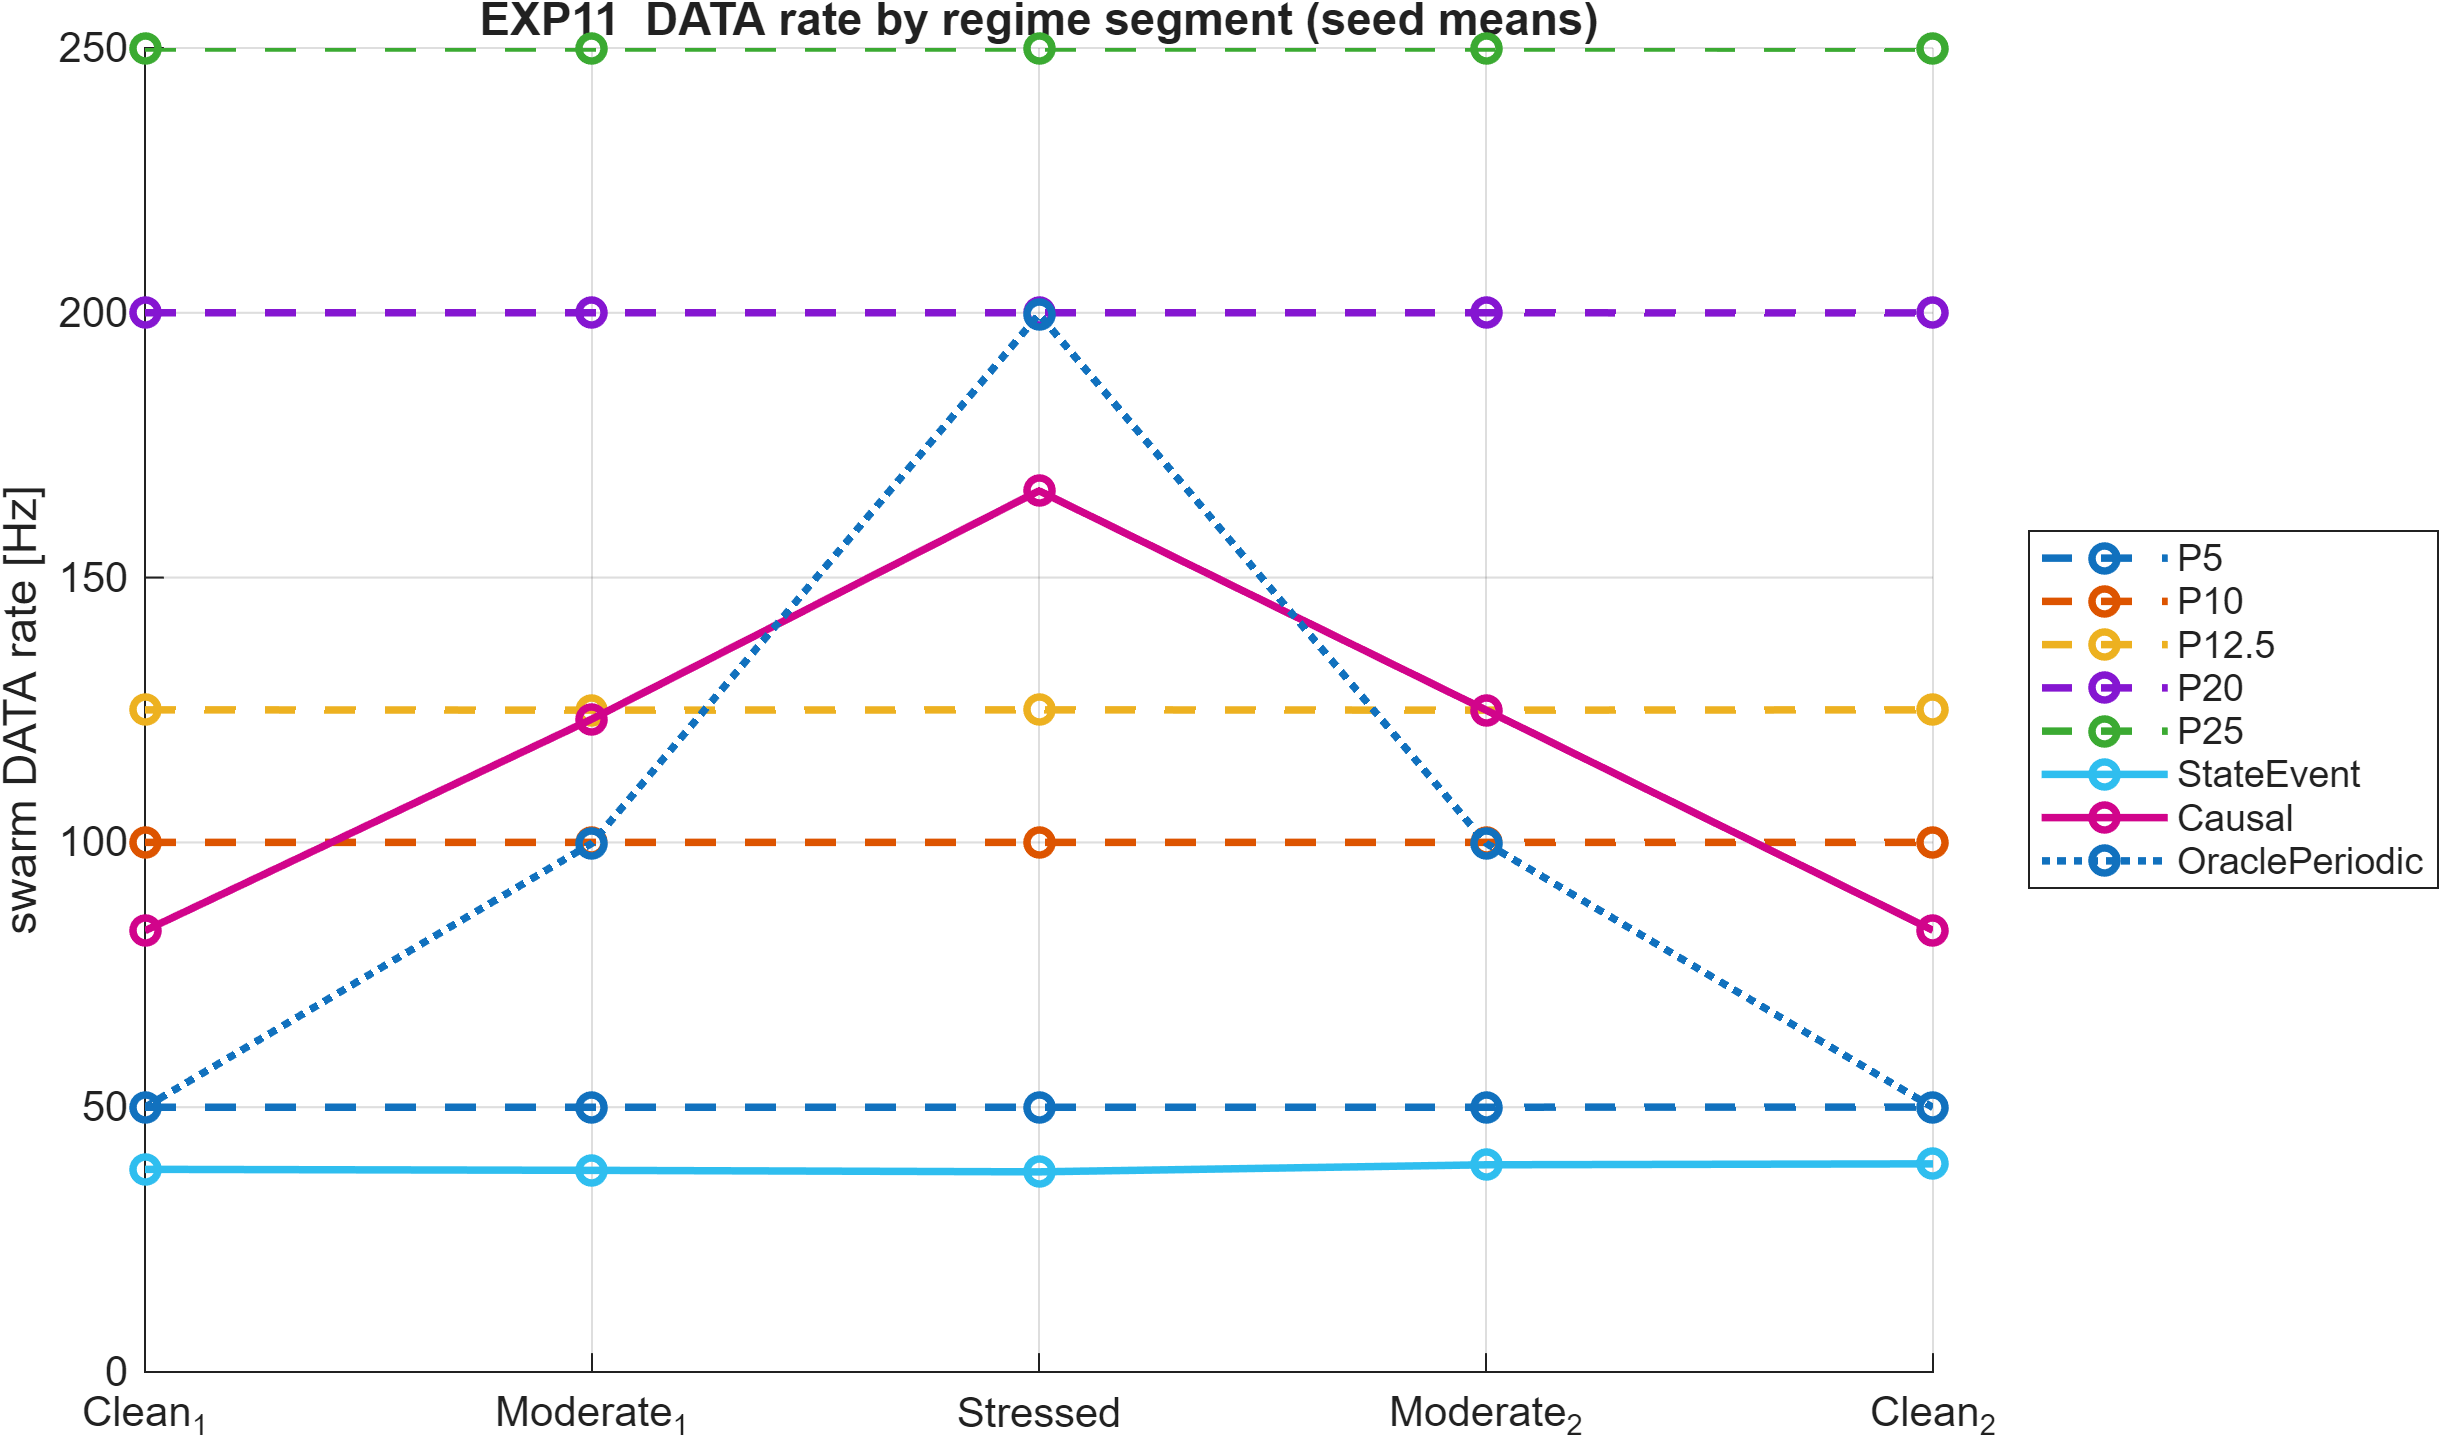
\includegraphics[width=0.78\textwidth]{fig12_exp11_adaptivity}
\caption{EXP11 within-run \textbf{swarm-total DATA rate}. The fixed causal
policy receives no regime label; all adjacent paired intervals have the
expected sign.}
\label{fig:exp11adaptivity}
\end{figure*}

H1 is supported: the four adjacent rate differences and all confidence
intervals appear in Table~\ref{tab:exp11claims}. H2a is supported:
RMSE(Causal$-$P10) is \MetricElevenHtwoaMean{} m
$[\MetricElevenHtwoaLo{},\MetricElevenHtwoaHi{}]$. H2b is supported only at preregistered $w=0.25$: $C_{0.25}$(Causal$-$P20) is
\MetricElevenHtwobMean{} Hz
$[\MetricElevenHtwobLo{},\MetricElevenHtwobHi{}]$. This is not general
ACK-inclusive superiority.

\begin{table}[t]
\centering
\caption{EXP11 frontier characterization. P12.5 is the counterexample to
universal mission-level dominance. Rates are swarm totals;
$C_{0.25}=$DATA$+0.25$ACK. Broadcast is the accounting proxy in
\eqref{eq:costbcast}, not an actual broadcast-medium simulation.}
\label{tab:exp11frontier}
\scriptsize
\resizebox{\columnwidth}{!}{\begin{tabular}{@{}lrrr@{}}
\toprule
Method & RMSE [m] & $C_{0.25}$ [Hz] & broadcast [Hz] \\
\midrule
P5 & \MetricElevenPfiveRmse{} & \MetricElevenPfiveCost{} & \MetricElevenPfiveBroadcast{} \\
P10 & \MetricElevenPtenRmse{} & \MetricElevenPtenCost{} & \MetricElevenPtenBroadcast{} \\
\textbf{P12.5} & \textbf{\MetricElevenPonetwofiveRmse{}} & \textbf{\MetricElevenPonetwofiveCost{}} & \textbf{\MetricElevenPonetwofiveBroadcast{}} \\
P20 & \MetricElevenPtwentyRmse{} & \MetricElevenPtwentyCost{} & \MetricElevenPtwentyBroadcast{} \\
P25 & \MetricElevenPtwentyfiveRmse{} & \MetricElevenPtwentyfiveCost{} & \MetricElevenPtwentyfiveBroadcast{} \\
State-event & \MetricElevenStateeventRmse{} & \MetricElevenStateeventCost{} & \MetricElevenStateeventBroadcast{} \\
\textbf{Causal-v3} & \textbf{\MetricElevenCausalRmse{}} & \textbf{\MetricElevenCausalCost{}} & \textbf{\MetricElevenCausalBroadcast{}} \\
Oracle-periodic\textsuperscript{*} & \MetricElevenOracleRmse{} & \MetricElevenOracleCost{} & \MetricElevenOracleBroadcast{} \\
\bottomrule
\multicolumn{4}{@{}l}{\footnotesize \textsuperscript{*}Non-causal, regime-aware oracle-information reference.}
\end{tabular}}
\end{table}

H3 and H4 are characterizations. P12.5 retains
\MetricElevenPonetwofiveAccuracyPercent{}\% of Causal-v3 accuracy at
\MetricElevenPonetwofiveCostPercent{}\% of its $C_{0.25}$ cost and
\MetricElevenPonetwofiveBroadcastPercent{}\% of its broadcast cost. Moreover,
broadcast(Causal$-$P20) is \MetricElevenBroadcastPtwentyMean{} Hz
$[\MetricElevenBroadcastPtwentyLo{},\MetricElevenBroadcastPtwentyHi{}]$,
a reversal of the favorable ACK-weighted comparison. The regime-aware
oracle-periodic information reference differs by
\MetricElevenOracleRmseMean{} m in RMSE and
\MetricElevenOracleCostMean{} Hz in $C_{0.25}$; it is an efficiency
reference, not a bound.

\subsection{R4: communication-cost limitation}
\begin{figure*}[t]
\centering
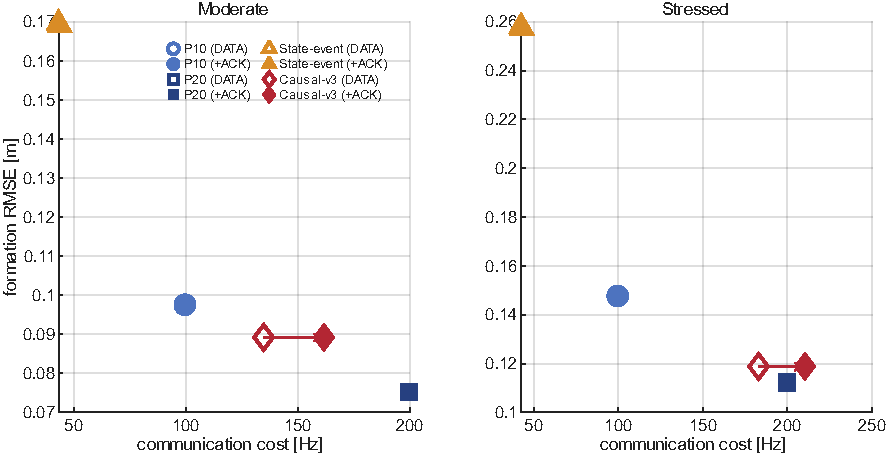
\includegraphics[width=0.72\textwidth]{fig05_cost_pareto}
\caption{Nominal accuracy versus \textbf{swarm-total} communication cost.
Hollow markers count DATA; filled markers add $0.25$ACK. ACK pricing moves
Causal-v3 across P20 in the Stressed panel.}
\label{fig:pareto}
\end{figure*}

Under $w=0.25$, Causal-v3 is non-dominated in
\MetricParetoModerateWtwentyfive{}\% of Moderate point families, satisfying
the preregistered criterion. The corresponding Stressed Pareto claim was
rejected. At
$w=0.50$, airtime, and broadcast accounting, the Stressed non-dominance rates
remain only \MetricParetoStressedWfifty{}\%,
\MetricParetoStressedAirtime{}\%, and \MetricParetoStressedBroadcast{}\%.
The policy is cheapest in \MetricCausalCheapestCells{} of
\MetricTotalCells{} cells. These negative results rule out a general
reduction in total radio traffic.

\subsection{R5--R6: 6-DOF survival and operating boundaries}
\begin{figure*}[t]
\centering
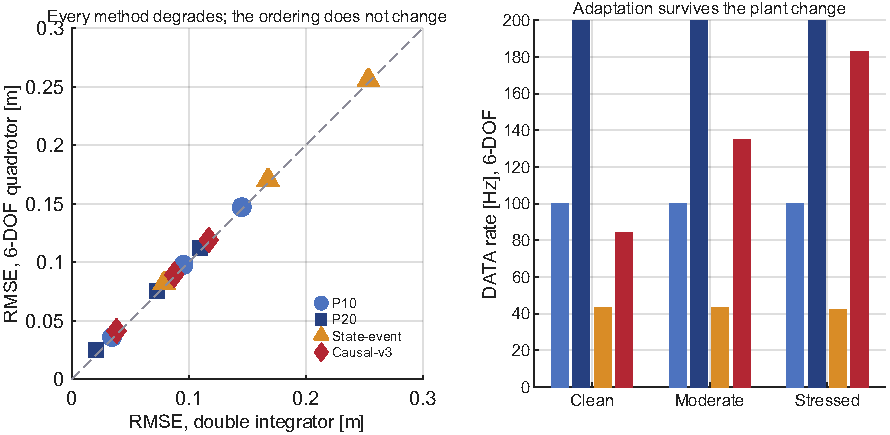
\includegraphics[width=0.68\textwidth]{fig09_di_vs_6dof}
\caption{Simulation-only comparison of double-integrator and 6-DOF followers
at $N=5$. Accuracy degrades for all methods, while ordering and the adaptive
rate response survive.}
\label{fig:sixdof}
\end{figure*}

The transition to 6-DOF quadrotors degrades every method but retains method
ordering and adaptivity. Broader sweeps identify boundaries rather than a
universal robustness claim. In the Stressed reverse-channel sweep, reliable
and impaired ACKs both give \MetricAckImpStressedReliableRate{} Hz with a mean
adaptive scale of \MetricAckImpStressedReliableScale{}, near the configured
$s_{\min}=0.20$ floor; the flat response is saturation, not robustness. By
contrast, in Moderate conditions the mean scale falls from
\MetricAckImpModerateReliableScale{} to
\MetricAckImpModerateImpairedScale{} as the DATA rate rises from
\MetricAckImpModerateReliableRate{} to
\MetricAckImpModerateImpairedRate{} Hz. One topology condition fails because
the consensus gain is not degree-normalized; permanent link removal and node
blackout create shared controller/geometry failures; mass mismatch leaves
steady error without integral action; estimator noise creates false
hard-innovation triggers; and traffic depends on the sampled outer step.

\begin{table*}[t]
\centering
\caption{Negative and boundary results retained in the main paper. Each row
records a tested claim that was rejected or bounded. Rate units follow the
source experiment: EXP07 is per channel, whereas EXP08+ is swarm total; values
must not be compared across those conventions.}
\label{tab:negative}
\scriptsize
% Table VI -- negative and boundary results. GENERATED, do not edit.
% This table must not be removed or shortened: it is the record
% that these claims were tested and did not hold.
\begin{tabular}{p{4.1cm}lp{5.0cm}p{4.4cm}}
\toprule
Rejected or bounded claim & Source & Frozen evidence & Attribution \\
\midrule
Stressed ACK-inclusive Pareto superiority & EXP07C, EXP10B & Stressed non-dominated in 38\% of cells at $w=0.50$, airtime and broadcast & ACK traffic is real traffic; pricing it removes the advantage \\
\addlinespace
Universal topology safety & EXP08A & safety gate fails systematically at one condition of the topology sweep & unnormalised consensus gain scales with in-degree (EXP08A-D) \\
\addlinespace
Absolute safety under permanent link failure & EXP08B, EXP10B & EXP10 20\% removal, Moderate: unsafe 9/49 for P10, P20 and Causal alike & formation geometry and controller, not the communication policy \\
\addlinespace
Safety under a 5\,s node blackout & EXP08C, EXP10B & EXP10, matched no-fault eligibility: unsafe 9/50 (Causal) & a dark node cannot be reached by any policy \\
\addlinespace
$\le 25\%$ RMSE degradation under B7 mismatch & EXP09B, EXP10B & EXP10 Moderate: 0.7317 vs 0.0892 nominal, $+720\%$ & no integral action: a mass offset leaves a steady error \\
\addlinespace
Clean estimator-noise traffic $<2\times$ & EXP09C & Clean DATA ratio $\times2.34$ against the noiseless arm & measurement noise itself crosses the hard-innovation threshold \\
\addlinespace
DATA-rate invariance to $\Delta t$ & EXP09C-dt & Stressed DATA 202.9 / 182.9 / 133.0 Hz at $\Delta t=$ 0.01 / 0.02 / 0.04 s & the trigger is evaluated once per outer step by construction \\
\addlinespace
\bottomrule
\end{tabular}

\end{table*}

Across all \MetricRuns{} final-validation runs, there were
\MetricDiverged{} divergences and \MetricInvariants{} protocol-invariant
violations. All registered realization hashes and matched seed assignments
passed the frozen-data audit.

\section{Discussion}
\label{sec:discussion}

\subsection{Mechanism versus mission-level superiority}
The design chain supports a causal account. Ideal receiver knowledge exposes
redundant in-flight retransmission; lastSent/lastAcked dual memory removes that
ambiguity; v2 then reveals over-suppression because one cooldown governs both
innovation and repetition. V3 resolves the semantic conflict by prioritizing
new information and suppressing only refresh. The rate response in EXP10 and
the four signed transitions in EXP11 support mechanistic adaptivity.

That result is not the same as Pareto superiority. A fixed periodic scheduler
cannot adapt its communication effort to within-mission network changes because
its rate is invariant by construction; however, a well-selected fixed rate can
still provide a competitive mission-level accuracy--cost trade-off. P12.5 is
the concrete counterexample: it retains
\MetricElevenPonetwofiveAccuracyPercent{}\% of Causal-v3 accuracy at
\MetricElevenPonetwofiveCostPercent{}\% of its ACK-weighted cost and
\MetricElevenPonetwofiveBroadcastPercent{}\% of its broadcast cost. EXP11
therefore supports the adaptation mechanism, not universal superiority.

\subsection{Why accounting changes the conclusion}
Periodic baselines require no modeled reverse ACK channel, while Causal-v3
does. DATA-only accounting answers whether the policy sends fewer state
packets; $C_w$ answers whether that remains true after pricing feedback; the
broadcast model additionally credits one simultaneous medium transmission
rather than charging each receiver link. K2 and EXP11 show that favorable
DATA or ACK-weighted comparisons can reverse under another legitimate traffic
convention. Claims must therefore name the unit and accounting model.

\subsection{What the references and boundaries mean}
The ideal-feedback and oracle-periodic policies are ideal-feedback,
oracle-information, or efficiency references. They are not bounds on
attainable accuracy or performance. Similarly, the robustness sweeps characterize where
the fixed causal mechanism operates: saturation, controller degree scaling,
unrecoverable blackouts, mass offset, estimator-triggered traffic, and sampled
timestep dependence. They do not establish stability or universal robustness.

\section{Limitations}
\label{sec:limitations}

This work is simulation-only and has no hardware validation. The 6-DOF plant
is a validation model, not evidence of flight deployment; the estimator,
disturbance, radio, and traffic models are synthetic rather than claims of
sensor or aerodynamic realism.

The evidence does not support universal superiority over tuned periodic
communication, general ACK-inclusive savings, or a broadcast-medium advantage.
P12.5 remains highly competitive, the Stressed ACK-inclusive Pareto claim is
rejected, and the favorable EXP11 P20 comparison holds only at preregistered
$w=0.25$. One changing mission characterizes adaptivity but cannot cover all
mission schedules or networks.

The formation controller is not redesigned here. Consequently, degree-scaled
gain, permanent disconnection, blackout, and steady mass-offset failures are
not repaired by the communication layer. Likewise, fixed innovation thresholds
react to estimator noise, and transmission rate depends on the sampled outer
step. Table~\ref{tab:negative} keeps these operating boundaries visible.

Finally, sampled evaluation excludes Zeno transmissions by construction, but
neither this property nor the empirical safety gates constitute a closed-loop
stability proof. Generalization to other graphs, missions, swarm sizes,
hardware radios, and controllers remains to be tested.

\section{Conclusion}
\label{sec:conclusion}

We presented a causal ACK-assisted, AoI-aware event-triggered
communication policy for multi-UAV formation control. The sender estimates
receiver freshness only from cumulative acknowledgements crossing a
delayed and lossy reverse channel, keeps that estimate in a memory
separate from the last state it transmitted, and --- the element the design
history turns on --- distinguishes traffic that carries new information
from traffic that merely repeats it, so that a repetition cooldown governs
only repetition.

On a pre-registered holdout validation over \MetricSeeds{} unseen seeds
and \MetricRuns{} runs, one fixed configuration adapts its DATA traffic
monotonically with network quality
(\MetricDataCausalClean{} $<$ \MetricDataCausalModerate{} $<$
\MetricDataCausalStressed{}~Hz), attains lower formation error than a
conventional state-event trigger in all \MetricTotalCells{} cells of the
final matrix, and improves on a $10$~Hz periodic baseline in the Stressed
condition by \MetricKoneMean{}~m with a $95\%$ interval of
$[\MetricKoneLo{}, \MetricKoneHi{}]$. In the Moderate condition it is
non-dominated in \MetricParetoModerateWtwentyfive{}\% of the selected
point families under the reference cost model. The design-evolution
ablation isolates why each element is needed: a fixed threshold does not
adapt, adaptation on an open loop adapts in the wrong direction, and
closing the loop without separating the two traffic semantics pins the
rate so that the policy cannot perceive a worse network at all.

The boundaries are as much of the result as the improvements, and three
deserve repeating in a conclusion rather than being left in a limitations
section.

First, \textbf{the saving is a DATA-packet saving.} Against $20$~Hz
periodic the paired DATA difference is \MetricKtwoaMean{}~Hz and the
ACK-inclusive difference is \MetricKtwobMean{}~Hz, both with intervals
excluding zero. The policy's contribution is adaptivity and accuracy, not
a reduction in total radio traffic, and under the reference cost model it
is the cheapest method in \MetricCausalCheapestCells{} of
\MetricTotalCells{} cells.

Second, \textbf{an acausal oracle is an information-efficiency
reference, not an accuracy bound.} The oracle variant transmits less
(\MetricSevenIdealStressedRate{}~Hz per channel) and is \emph{less}
accurate (\MetricSevenIdealStressedRmse{}~m) than the causal policy
(\MetricSevenAfivecStressedRate{}~Hz, \MetricSevenAfivecStressedRmse{}~m).
Perfect freshness knowledge mainly buys the confidence to stay quiet.

Third, \textbf{several failures the campaign found are not communication
failures.} A steady offset under mass mismatch, a degree-dependent safety
boundary, and safety failures under link and node faults that are
identical across all four methods all belong to the control layer. We
report them, attribute them, and do not claim to have addressed them.

\subsection*{Future work}

The results point to specific next steps rather than general ones.

\emph{Reverse-channel cost} is the sharpest lever: aggregating
acknowledgements across links, or piggybacking them on data a node is
already sending, would attack the one cost model under which the method is
clearly unfavourable.

\emph{Broadcast alignment} follows from the same analysis. The policy
already sends one payload per sender to all its listeners; aligning
transmissions across senders would recover part of the broadcast-accounting
gap.

\emph{Noise-aware triggering} addresses the estimator boundary directly:
the innovation test should respond to motion in excess of measurement
uncertainty rather than to the raw norm, which is what caused the
factor-of-\MetricCleanNoiseRatio{} Clean traffic increase.

\emph{Timestep-invariant formulation} would decouple trigger evaluation
from the control step so that a quoted rate is a property of the policy
rather than of $\Delta t$.

\emph{Hardware transition} is staged in
\texttt{docs/HARDWARE\_ROADMAP.md}, beginning with protocol emulation and
embedded timing rather than flight, because the assumptions most in need of
measurement --- packet sizes, serialisation latency, ACK round-trip
distribution, radio duty cycle --- can be tested on a bench before any
vehicle is involved.

\subsection*{Reproducibility}

The complete campaign is frozen at a tagged commit. One command re-runs
the test suite, re-verifies every random realisation against a registry
computed in advance, checks bit-identity between serial and parallel
execution, rebuilds every table and figure in this paper from persisted
result files, and writes an environment manifest. A separate check clones
the repository and reproduces the test suite, the aggregate tables and one
re-simulated seed bit-identically. Every number in this paper is a
generated macro traceable to a named result directory; none is typed into
the prose.


\appendix

\section{Reproducibility}
The complete claim ledger, the frozen result directories behind every
number, and the single-command validation entry point are documented in
\texttt{paper/REPRODUCIBILITY.md} and \texttt{docs/FINAL\_CLAIMS.md} of
the accompanying repository, at tag \texttt{simulation-v1.0}.

\end{document}
